\scanpage{69}\mspage{68}
% First paragraph; the two additions and their distinct connecting strokes are kept in this local group.
% figure R1-F1
\figure{%
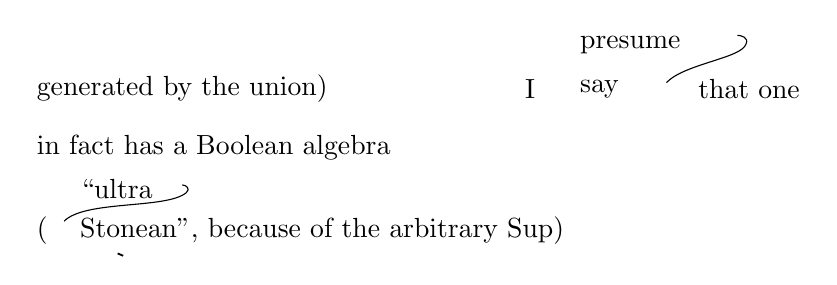
\begin{tikzpicture}[x=1cm,y=1cm]
  \node[anchor=west] at (0,1.8) {generated by the union)};
  \node[anchor=west] at (6.2,1.8) {I};
  \node[anchor=west] at (6.9,1.8) {\deleted{say}};
  \node[anchor=west] at (8.4,1.8) {that one};
  \node[anchor=west] at (6.9,2.35) {\inserted{presume}};
  \draw (8.12,1.88) .. controls (8.35,2.12) and (9.08,2.19) .. (9.13,2.37) .. controls (9.17,2.45) and (9.07,2.48) .. (9.02,2.48);
  \node[anchor=west] at (0,1.05) {in fact has a Boolean algebra};
  \node[anchor=west] at (0,0) {(};
  \node[anchor=west] at (0.55,0) {Stonean'', because of the arbitrary $\mathrm{Sup}$)};
  \node[anchor=west] at (0.55,0.53) {\inserted{``ultra}};
% Detached short stroke below stonienne; no function is assigned.
  \draw[line width=0.65pt] (1.15,-0.29)--(1.22,-0.32);
  \draw (0.47,0.12) .. controls (0.74,0.39) and (1.76,0.27) .. (2.02,0.48) .. controls (2.08,0.53) and (2.02,0.58) .. (1.97,0.58);
\end{tikzpicture}%
}
% slanted left margin note
\margin{This will be valid in ``the set-theoretic case'', and in any case in the typical examples, given \deleted{\unsure{right}} at the beginning, in terms of an $E$ (topological or measurable), then $\Sigma$ is identified with the set of subsets of $E$, and \unsure{one finds|one will find|one finds again} the \unsure{Stone} compactification of $E_{\mathrm{disc.}}$ In the case that follows, \unsure{I} \unsure{do not see} how to \unsure{prove}, for three supports
\[P,Q,R\quad P\wedge(Q\vee R)=\unsure{\{|(}(P\wedge Q)\vee(P\wedge R)\unsure{\}|.|,|)}\]}

\deleted{It will be necessary to return to this}

\unsure{Thus} the supports \unsure{are identified|would be identified} with the \unsure{Subsets|Subset} both open and closed in the spectrum, which would be a \deleted{\unsure{to|totally}}\unsure{compact|compact|compact} \deleted{\unsure{totally}} \unsure{disconnected} ultra.Stonean space.

The involution corresponds to passage to the complement.

% Construction paragraph with the two insertion leaders; words occur once.
% figure R1-F2
\figure{%
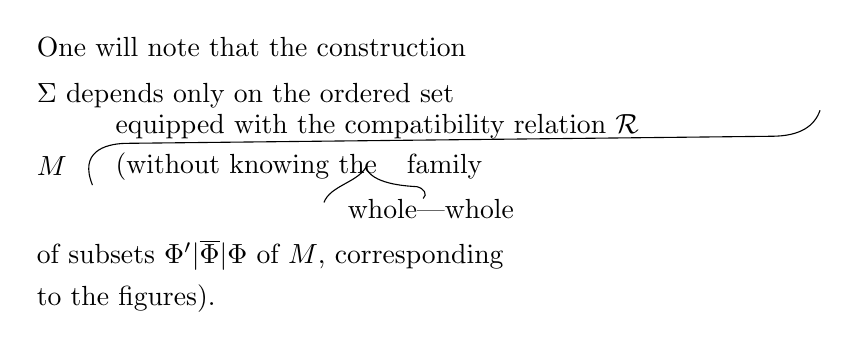
\begin{tikzpicture}[x=1cm,y=1cm]
  \node[anchor=west] at (0,2.0) {One \unsure{will} note that the construction};
  \node[anchor=west] at (0,1.38) {$\Sigma$ depends only on the ordered set};
  \node[anchor=west] at (0,0.48) {$M$};
  \node[anchor=west] at (1.0,0.48) {(without knowing the};
  \node[anchor=west] at (4.7,0.48) {family};
  \node[anchor=west] at (1.0,0.98) {\inserted{equipped with the compatibility relation $\mathcal R$}};
  \draw (0.83,0.24) .. controls (0.66,0.66) and (0.98,0.76) .. (1.24,0.77) -- (9.45,0.86) .. controls (9.82,0.86) and (10.00,0.99) .. (10.07,1.19);
  \node[anchor=west] at (3.95,-0.06) {\inserted{\unsure{whole|whole}}};
  \draw (3.77,0.02) .. controls (3.85,0.23) and (4.18,0.27) .. (4.30,0.46) .. controls (4.39,0.26) and (4.77,0.23) .. (4.95,0.22) .. controls (5.04,0.20) and (5.09,0.12) .. (5.03,0.07);
  \node[anchor=west] at (0,-0.65) {of subsets $\unsure{\Phi'|\overline\Phi|\Phi}$ of $M$, corresponding};
  \node[anchor=west] at (0,-1.20) {to the figures).};
\end{tikzpicture}%
}
Indeed, in terms of $(M,\leq,R)$, the cosupport of a subset $M'$ of $M$ is defined by
\[
\operatorname{cosup}_M(M')=\{\,x\in M\mid(x,x')\in\mathcal R\quad\forall x'\in\unsure{M'|M''}\,\}
\]
% Slanted bottom margin note and its long attached rule; no arrowhead is supplied.
% figure R1-F3
\figure{%
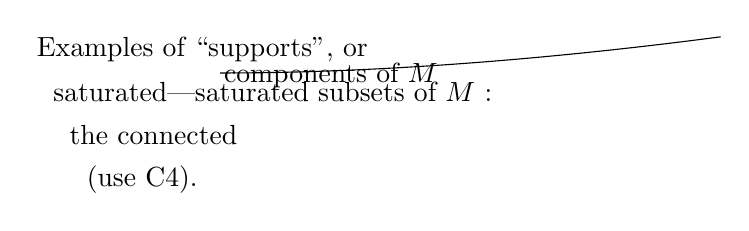
\begin{tikzpicture}[x=1cm,y=1cm]
\begin{scope}[rotate=21]
  \node[anchor=west] at (0,0) {\uline{Examples} of ``supports'', or};
  \node[anchor=west] at (0,-0.58) {\unsure{saturated|saturated} subsets of $M$ :};
  \node[anchor=west] at (0,-1.16) {the connected};
  \node[anchor=west] at (2.10,-1.16) {components of $M$};
  \node[anchor=west] at (0,-1.77) {(use C4).};
  \draw (2.18,-1.16) .. controls (4.23,-1.95) and (6.45,-2.57) .. (8.28,-3.01);
\end{scope}
\end{tikzpicture}%
}
